% Chapter Template

\chapter{Preliminary Results} % Main chapter title

\label{ch:results} % Change X to a consecutive number; for referencing this chapter elsewhere, use \ref{ChapterX}

\lhead{Chapter 4. \emph{Results}} % Change X to a consecutive number; this is for the header on each page - perhaps a shortened title

We consider some results from applying the methods described in Chapter \ref{ch:methods} to the physical
models outlined in Chapter \ref{ch:models}, organized by model.
%----------------------------------------------------------------------------------------
%	SECTION 1
%----------------------------------------------------------------------------------------

\section{Polynomial Evaluations}
Using an analytic polynomial evaluation as our model allows observation of best-case performance of SCgPC for
several dimensions.

\begin{figure}[H]
  \centering
    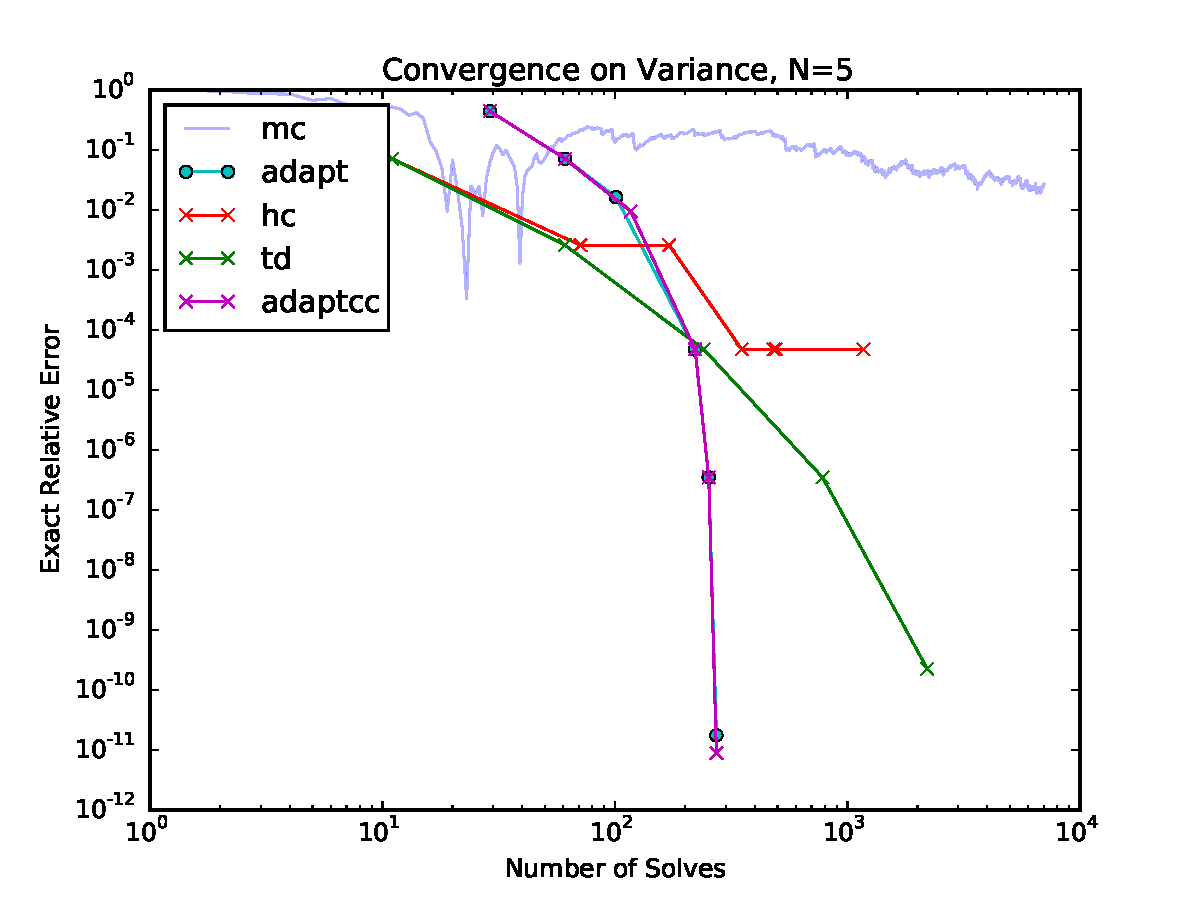
\includegraphics[width=0.7\linewidth]{./analytic5/anl_rand_varconv_5}
    \rule{35em}{0.5pt}
  \caption{Analytic $N=5$ Error Convergence, Variance}
  \label{fig:anl5_varconv}
\end{figure}
\begin{figure}[H]
  \centering
    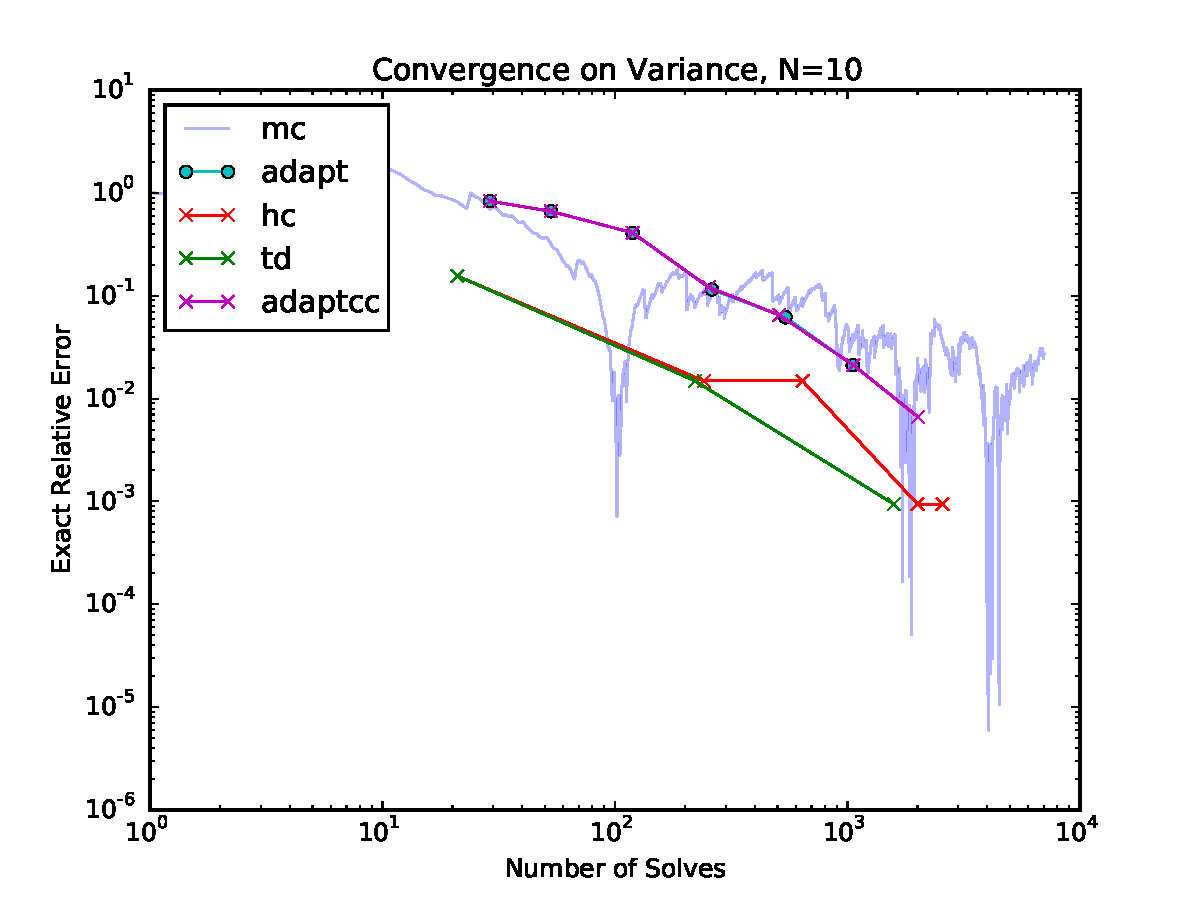
\includegraphics[width=0.7\linewidth]{./analytic10/anl_rand_varconv_10}
    \rule{35em}{0.5pt}
  \caption{Analytic $N=10$ Error Convergence, Variance}
  \label{fig:anl10_varconv}
\end{figure}



\section{Attenuation}

\begin{figure}[H]
  \centering
    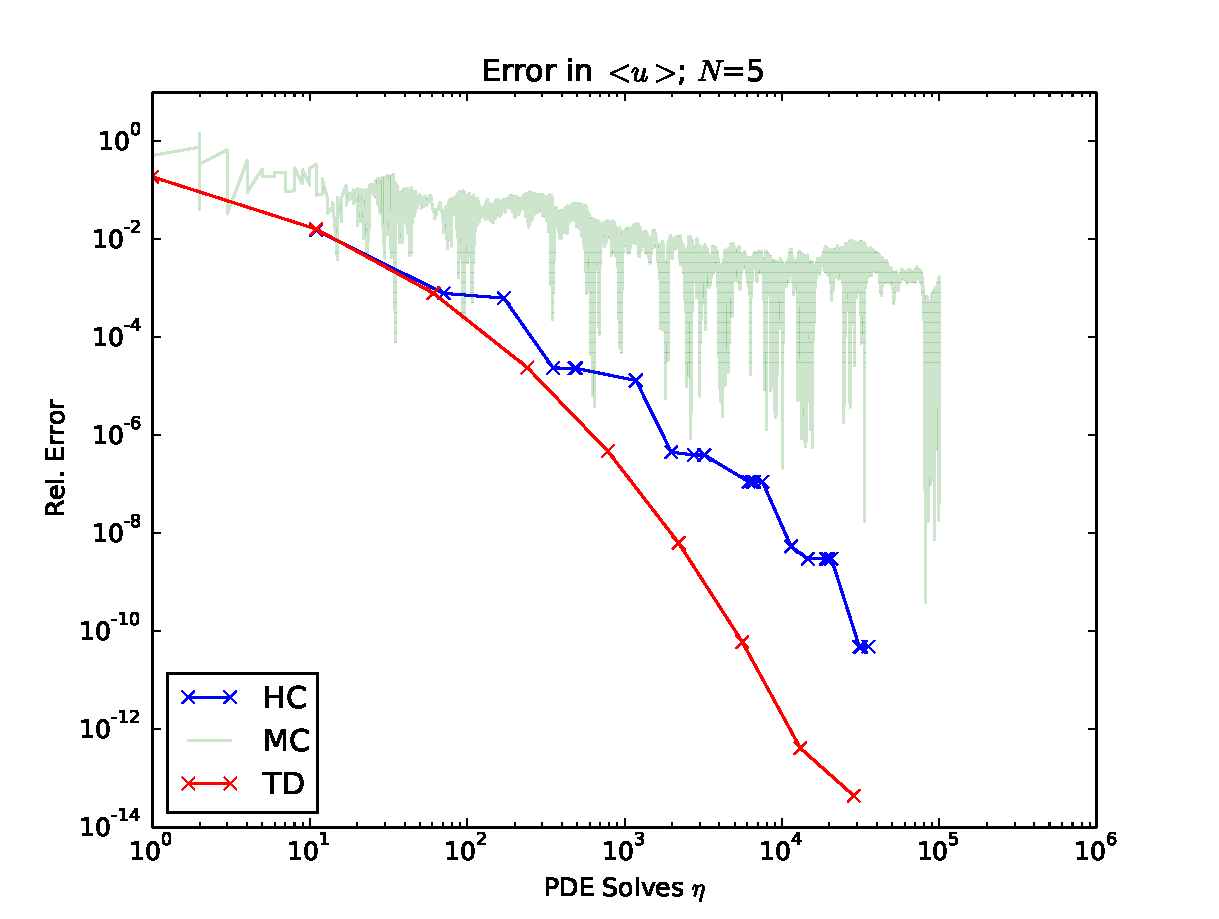
\includegraphics[width=0.7\linewidth]{attenuate_N5_conv}
    \rule{35em}{0.5pt}
  \caption{Attenuation $N=5$ Error Convergence, Variance}
  \label{fig:att5_varconv}
\end{figure}




\section{Projectile}

\begin{figure}[H]
  \centering
    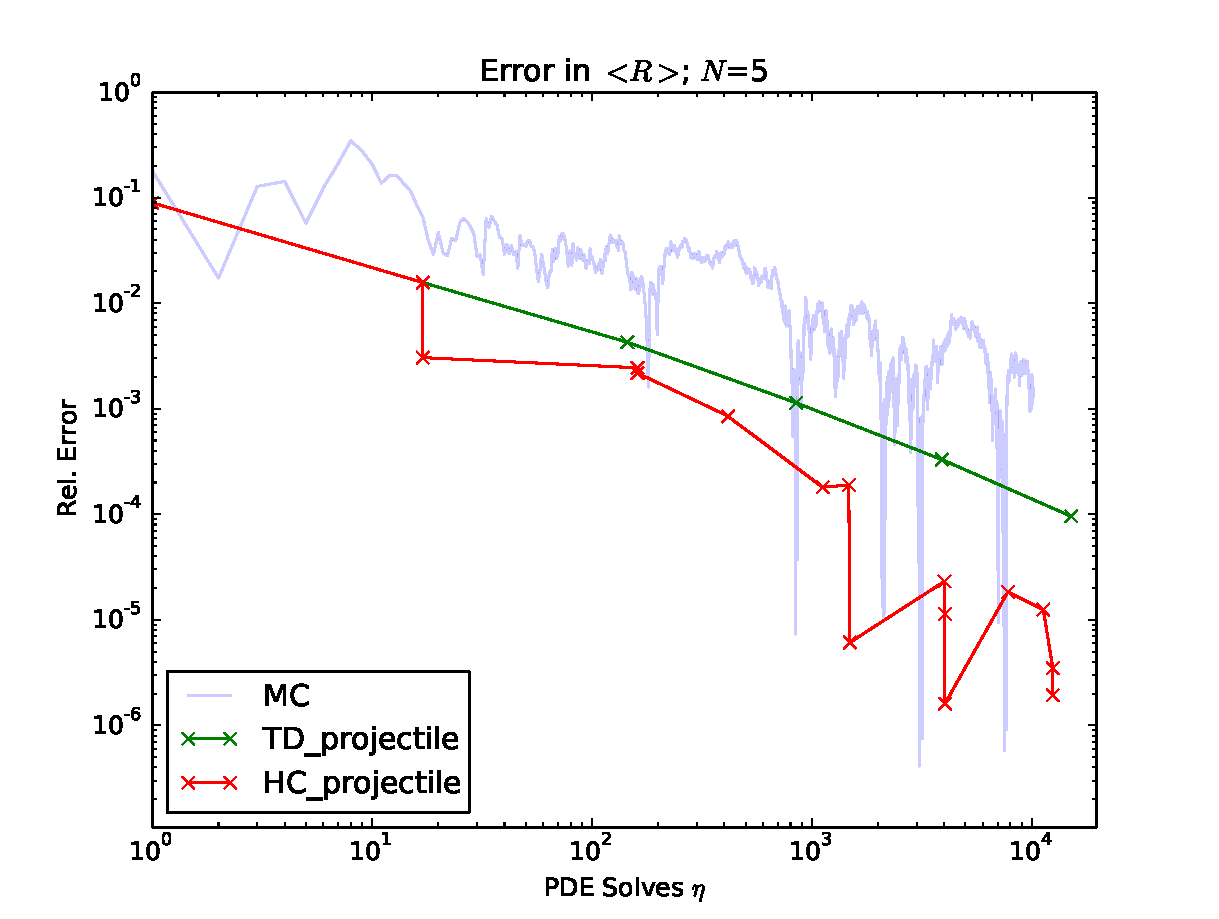
\includegraphics[width=0.7\linewidth]{projectile_errs}
    \rule{35em}{0.5pt}
  \caption{Projectile $N=8$ Error Convergence, Variance}
  \label{fig:proj_varconv}
\end{figure}



\section{Neutron Diffusion}

\begin{figure}[H]
  \centering
    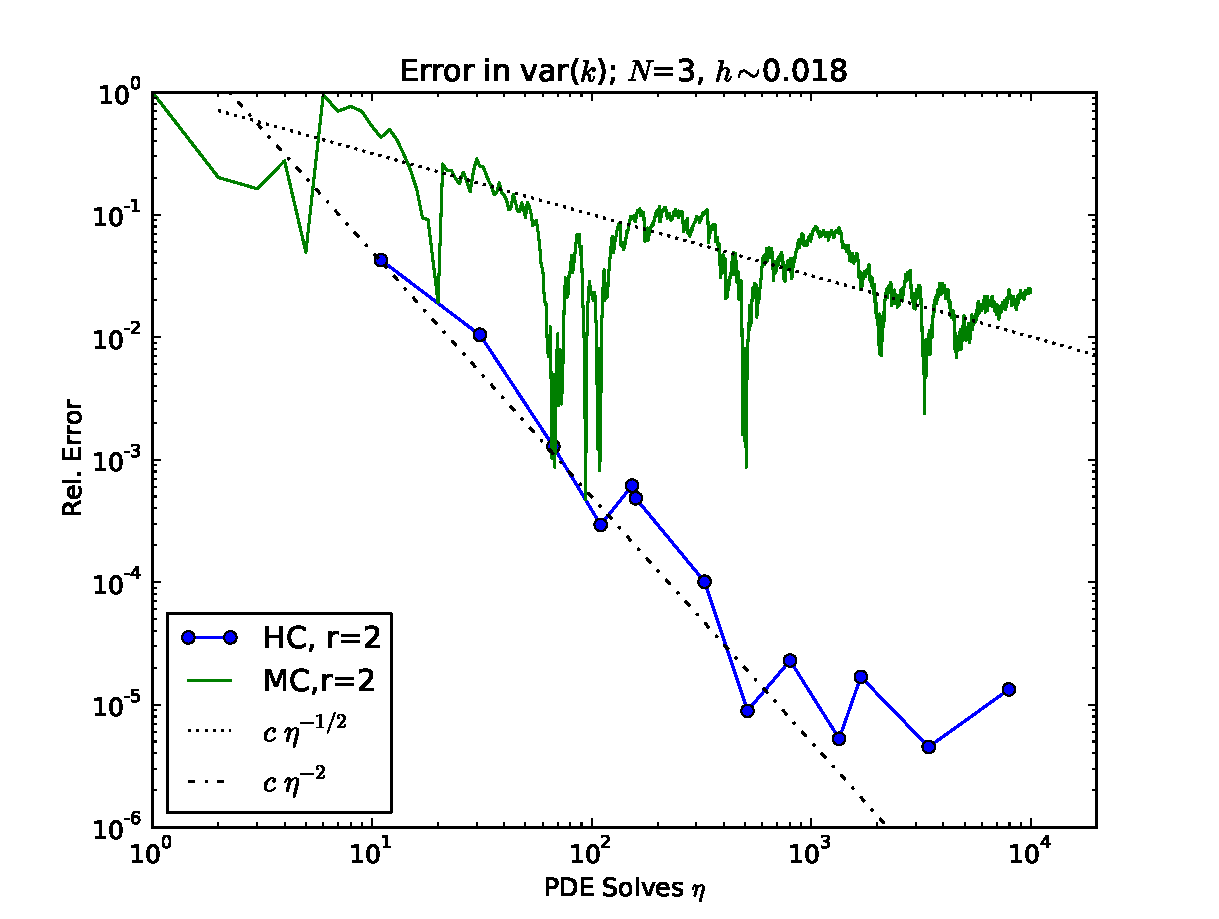
\includegraphics[width=0.7\linewidth]{N3_h5_MCHC_2}
    \rule{35em}{0.5pt}
  \caption{Diffusion $N=3$ Error Convergence, Variance}
  \label{fig:diff3_varconv}
\end{figure}
\begin{figure}[H]
  \centering
    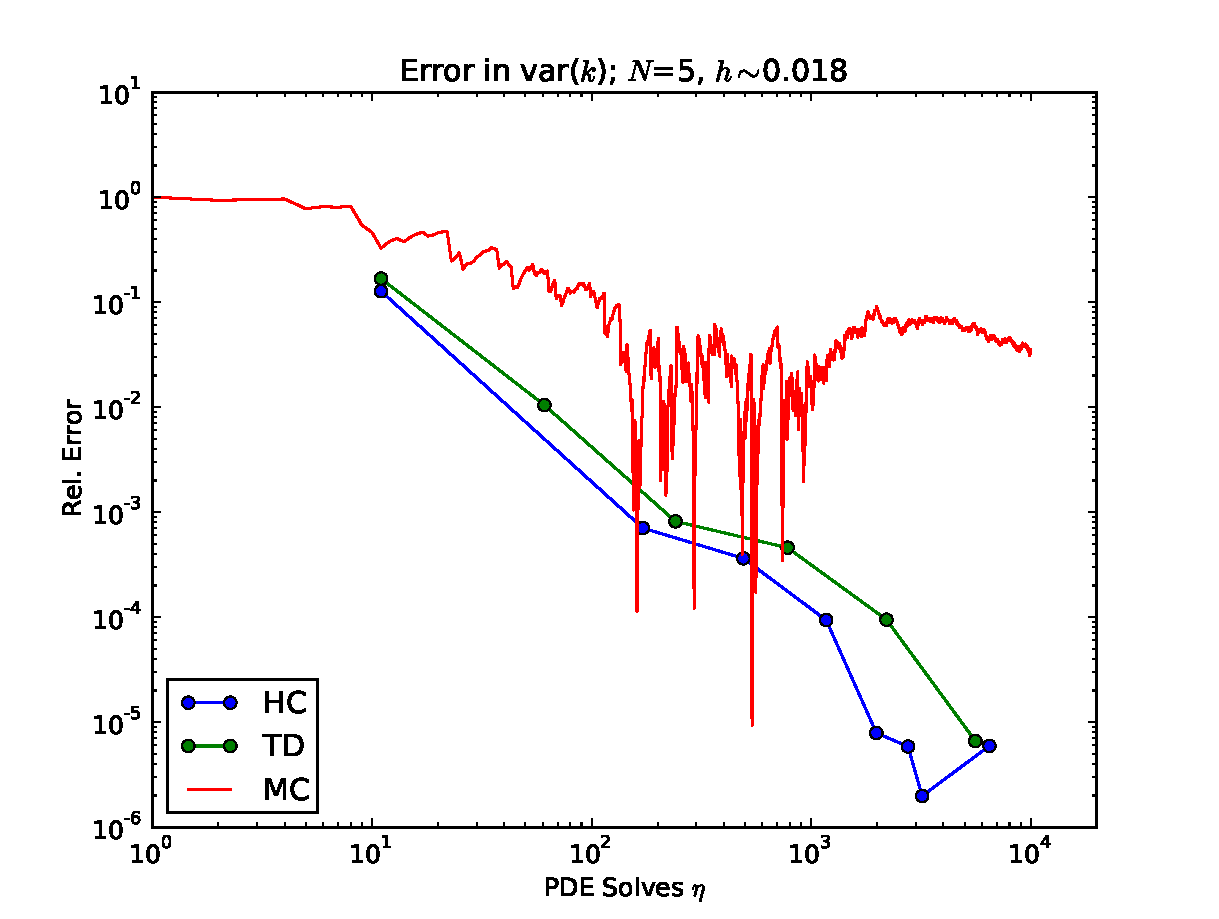
\includegraphics[width=0.7\linewidth]{N5_h5_MCHC_2}
    \rule{35em}{0.5pt}
  \caption{Diffusion $N=5$ Error Convergence, Variance}
  \label{fig:diff5_varconv}
\end{figure}
\begin{figure}[H]
  \centering
    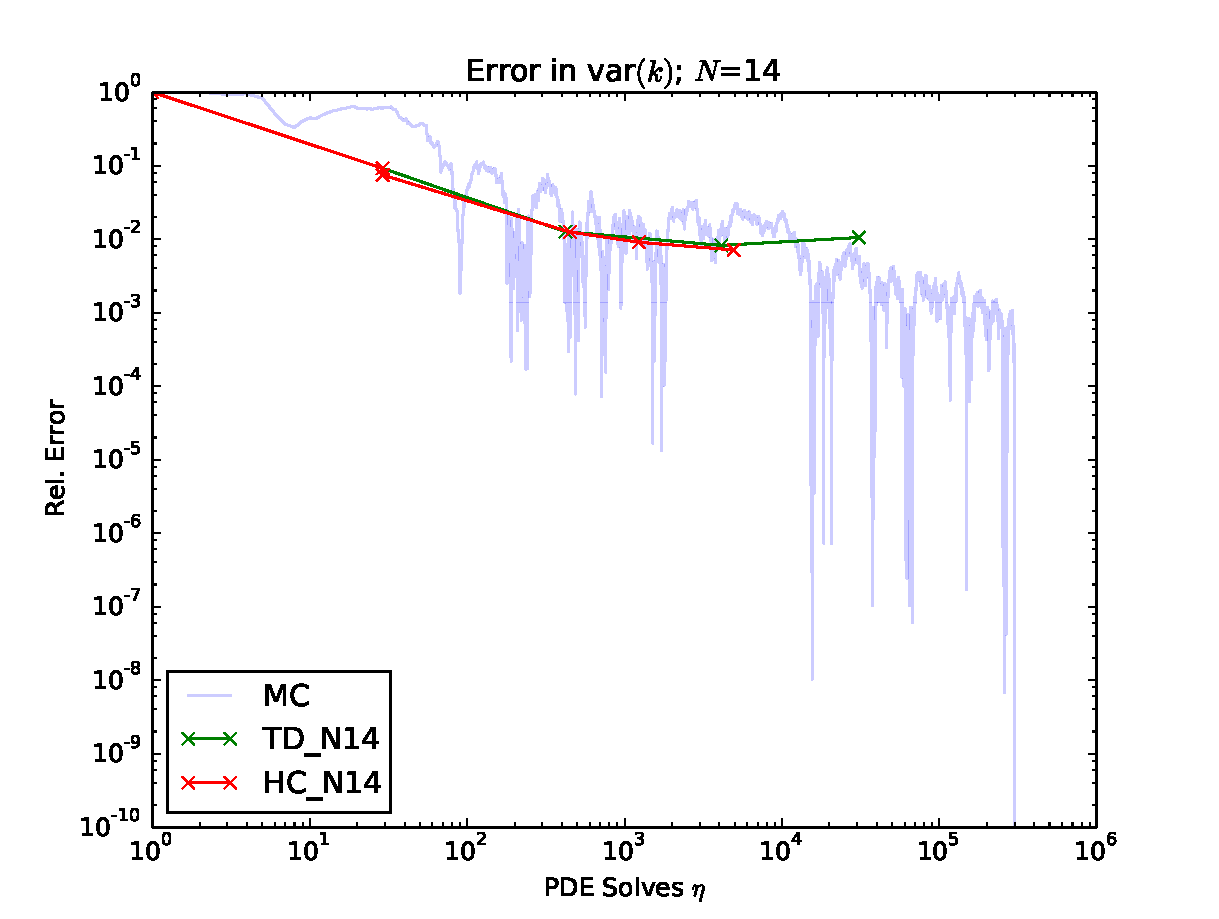
\includegraphics[width=0.7\linewidth]{N14_iso_var_errs}
    \rule{35em}{0.5pt}
  \caption{Diffusion $N=14$ Error Convergence, Variance}
  \label{fig:diff14_varconv}
\end{figure}





\section{Fuel Rod Performance}
todo

